\documentclass[a4paper, utf8]{ctexart}
\usepackage[fontset=Fandol]{ctex}
\usepackage{anyfontsize}
\usepackage{subcaption}
\usepackage{abstract}
\usepackage{appendix}
\usepackage{enumitem}
\usepackage{fancyhdr}
\usepackage{geometry}
\usepackage{graphicx}
\usepackage{amsmath}
\usepackage{caption}
\usepackage{lipsum}
\usepackage{minted}
\usepackage{pifont}
\usepackage{amsmath}

\geometry{a4paper,left=31mm,right=31mm,top=25mm,bottom=25mm}
\CTEXsetup[format={\Large \bfseries}]{section}
\setlength{\parindent}{2em}

\pagestyle{fancy}
\fancyhf{}
\fancyhead[C]{个人所得税计算器}
\fancyhead[L]{编译器构造实验}
\fancyhead[R]{Lab1设计文档}
\fancyfoot[C]{\thepage}
\fancyfoot[L,R]{}

\title{\songti \bfseries 个人所得税计算器\ 设计文档}
\author{\fangsong 傅祉珏\ \ 21307210}
\date{\fangsong 中山大学计算机学院\ 广东广州\ 510006}

\begin{document}

    \begin{titlepage}
        \centering
        \rule{\textwidth}{1pt}
        \vspace{0.02\textheight}

        {\LARGE \kaishu 编译器构造实验\ \ Lab1设计文档}

        \vspace{0.02\textheight}

        {\Huge \songti \bfseries 个人所得税计算器}

        \vspace{0.025\textheight}
        \rule{0.83\textwidth}{0.4pt}
        \vspace{0.05\textheight} 
        
        \begin{figure}[htbp]
            \centering
            
\includegraphics[width=8cm, height=8cm]{./figure/计院院徽.jpg}
        \end{figure}

        \vspace{0.05\textheight} 
        {\Large 课程编号:\textsc{DCS292}}

        \vspace{0.025\textheight} 
        {\Large 学生姓名:\textsc{傅祉珏}}

        \vspace{0.025\textheight} 
        {\Large 学生学号:\textsc{21307210}}

        \vspace{0.025\textheight} 
        {\Large 指导老师:\textsc{李文军\ 教授}}
 
        \vspace{0.025\textheight} 
        {\Large 项目截止日期:\textsc{2025年3月20日}}

        \vspace{0.05\textheight} 
        \vfill

        {\large \today}
        \vspace{0.1\textheight}
        \rule{\textwidth}{1pt}
    \end{titlepage}
    
    \let\cleardoublepage\clearpage

    \maketitle

    \renewcommand{\abstractname}{\large \textbf{摘要}}
    \begin{abstract}
        本报告介绍了一款可调整个人所得税起征点及税率表的计算器的设计与实现。系统采用分层架构,主要分为数据传输层、业务逻辑层和用户表示层,以模块化方式实现功能解耦和可维护性。数据传输层负责税收参数的数据存取,业务逻辑层执行税额计算,用户表示层提供直观的交互界面。此外,系统引入了异常处理机制,以提升用户输入的规范性和计算结果的准确性。

        通过核心功能测试、界面测试和异常处理测试,验证了系统的稳定性和计算准确性。实验结果表明,本系统能够在不同税率级别下正确计算税额,并具备较强的容错能力。然而,当前的数据存储仍依赖于本地文件,未来可考虑引入数据库或云存储,以提升系统的可扩展性。此外,未来版本可进一步优化税率更新机制,增强自动化程度。
	
        \noindent{\textbf{\heiti 关键词:}个人所得税,分层架构。}
    \end{abstract}

    \section{引言}

    个人所得税是国家对个人劳动所得征收的重要税种,其计算方式基于累进税率制度。根据中国现行《个人所得税法》,工资、薪金所得的应纳税额需通过以下步骤计算:首先,以月收入总额减去起征点及依法扣除的“三险一金”等专项费用,得到应纳税所得额;其次,根据超额累进税率表,将应纳税所得额按不同区间对应税率分段计算税款,最终累加得出应缴纳的个人所得税总额。

    随着社会经济的发展与政策调整,个人所得税法可能面临起征点、税率或扣除规则的修订(例如不同地区差异化执行标准或立法层面的基数调整)。为提升税务计算的灵活性与实用性,本项目旨在设计一款可自定义调整个人所得税起征点及税率表的个人所得税计算器应用程序。该程序核心功能包括:

    \begin{itemize}[itemsep=2pt, topsep=0pt, parsep=0pt]
        \item 工资薪金所得税计算:根据用户输入的月收入总额,自动完成应纳税所得额与税款的快速计算;
        \item 动态参数配置:支持通过配置文件或命令行菜单修改起征点、税率表等关键参数,以适配政策变化;
        \item 用户友好交互:通过简洁的GUI界面引导用户选择功能,降低操作门槛。
    \end{itemize}

    本项目的目标是为个人及小型企业提供轻量化的税务计算工具,同时通过模块化设计确保程序的扩展性与可维护性,为未来潜在的政策调整预留兼容性。

    \section{设计思路}

    基于项目目标的定位,本报告主要探讨系统架构设计方法论,而不涉及具体税收计算算法的数学推导。该项目采用分层架构设计,整体划分为用户表示层、业务逻辑层及数据传输层,以模块化方式实现功能解耦与可维护性。

    \begin{figure}
        \centering
        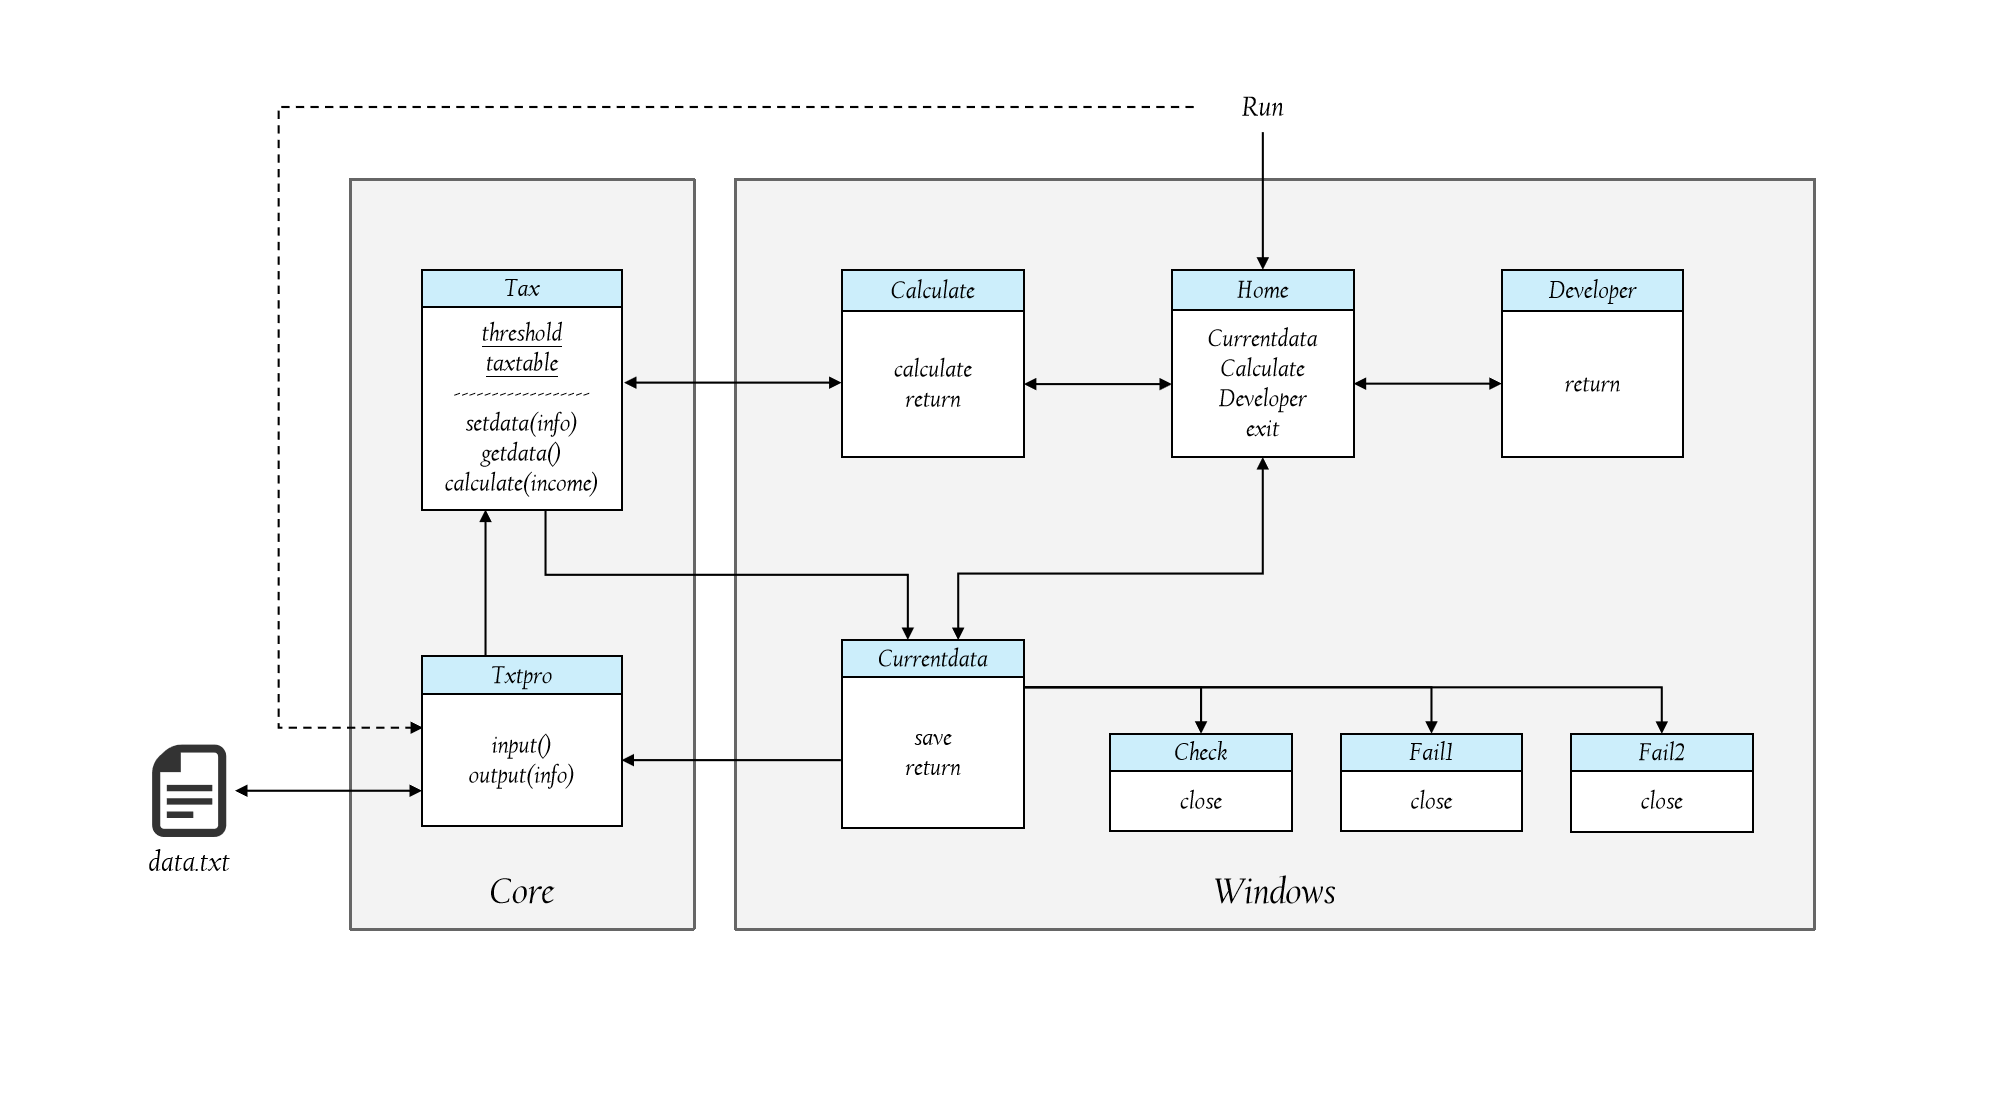
\includegraphics[width=0.95\linewidth]{figure/Structure.png}
        \caption{项目结构示意图}
    \end{figure}

    \subsection{数据传输层设计}

    数据传输层在数据存储文件与业务逻辑层之间承担桥梁作用,其主要职责包括从数据存储文件中读取信息并传递至业务逻辑层进行处理,同时接收业务逻辑层更新的数据并将其存储回数据存储文件。鉴于本系统需支持用户动态调整个人所得税起征点及税率表,数据传输层不仅负责数据的传输,还承担数据的持久化存储,以确保用户无需在每次程序启动时重新输入相关税收参数。
    
    \subsection{业务逻辑层设计}

    业务逻辑层是本项目的核心部分,仅由\verb|Tax|类构成。该类包含两个私有属性:个人所得税起征点和税率表。数据经由数据传输层导入\verb|Tax|类并存储,以作为计算个人所得税的依据。本项目未将税率表单独建模为一个独立类,主要是出于计算效率的考虑,以减少对象调用和时间开销,确保每次计算税款时仅使用已设定的单一税率表进行运算。如需使用其他税率表,则需重新输入新的个人所得税起征点及税率表参数。此外,为避免出现多个不同的税率计算实例,系统采用单例模式 (Singleton),确保\verb|Tax|类在程序运行期间仅实例化一次,从而保持计算逻辑的一致性。

    \subsection{用户表示层设计}

    用户表示层旨在提供直观、便捷的用户交互界面,使用户能够高效操作程序。本项目采用 JFrame 作为 GUI 组件,并设计了四个独立的界面以支持不同的功能:

    \begin{itemize}[itemsep=2pt, topsep=0pt, parsep=0pt]
        \item \verb|Home|界面:用户可在该界面选择跳转至其他功能界面。
        \item \verb|CurrentData|界面:用于查询当前的个人所得税起征点及税率表,并支持用户按照指定格式修改数据并进行保存。
        \item \verb|Calculate|界面:用于计算个人所得税。
        \item \verb|Developer|界面:用于显示开发者信息。
    \end{itemize}

    用户表示层在查询或修改数据时,需通过\verb|Tax|类提供的接口获取或存储数据,并在数据存储文件中进行持久化,以保证程序在下次启动时能够正确加载已保存的税收参数。

    \subsection{异常处理设计}

    在用户输入数据的过程中,可能会出现异常输入,若未加以处理,可能会导致程序崩溃。因此,本项目在用户表示层实现了异常处理机制,以阻断异常数据对业务逻辑层的影响,确保核心计算逻辑的稳定性。

    在\verb|Calculate|界面,用户输入的收入应为正数,系统将对输入值进行验证,以防止负数或非数值字符的输入,从而确保计算过程的正确性。在\verb|CurrentData|界面,个人所得税起征点同样需要为正数,而税率表的输入则需符合严格的格式要求。税率表的层级设定必须符合递增关系,即上一层级的下限不得大于下一层级的下限或上限,同时税率值和层级下界均应为正数。

    \begin{figure}[htbp]
        \begin{minipage}{.4\linewidth}
            \centering
            \vspace{.02\textheight}
            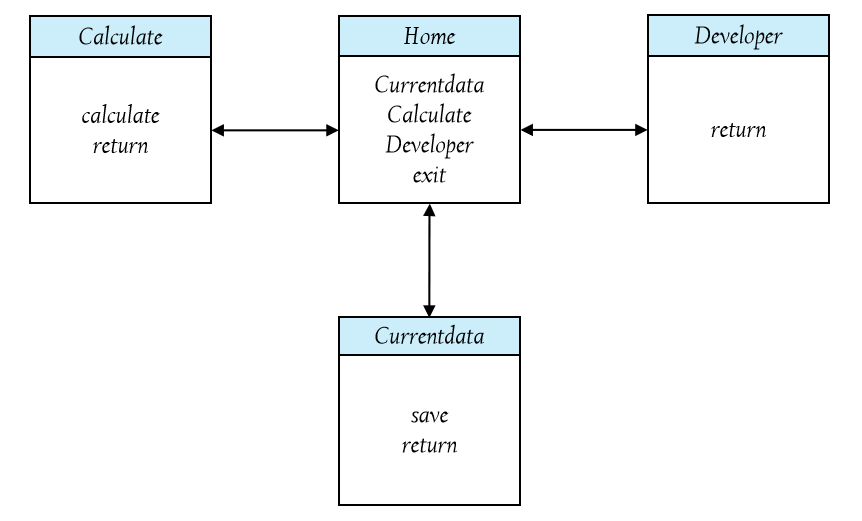
\includegraphics[height=0.13\textheight]{figure/Windows.png}
            \vspace{.02\textheight}
            \caption{GUI设计图}
        \end{minipage}
        \begin{minipage}{.6\linewidth}
            \centering
            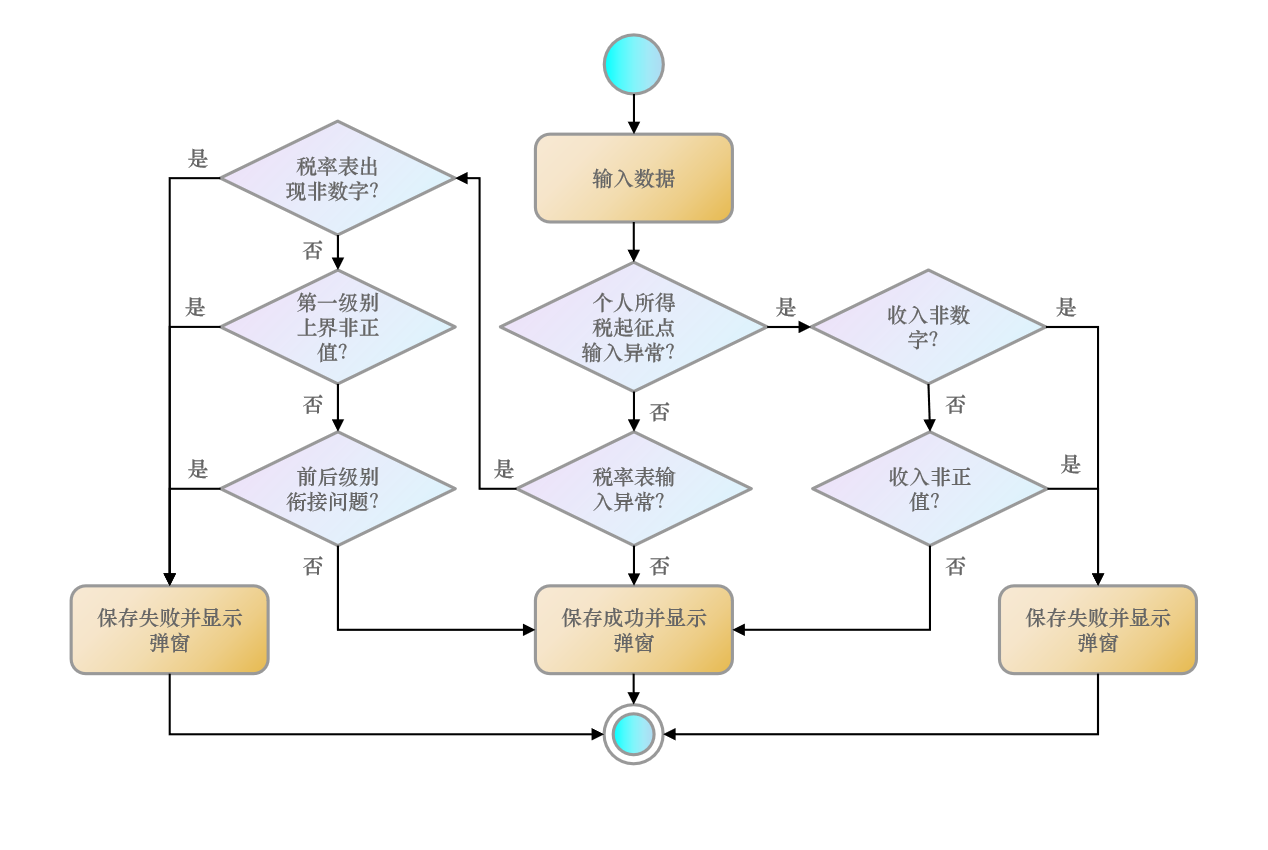
\includegraphics[height=0.17\textheight]{figure/Exception.png}
            \caption{异常处理流程示意图}
        \end{minipage}
    \end{figure}

    由于税率表的输入规则较为复杂,其异常处理机制较其他输入项更为严格和完善。系统不仅对输入格式进行校验,还会检测层级顺序的合理性,以确保税率计算的准确性和逻辑一致性。通过上述异常处理设计,本系统能够有效降低因用户输入错误而导致的计算偏差或程序崩溃的风险,从而提升系统的稳定性与用户体验。

    \section{实验测试}

    基于系统设计和用户需求分析,本项目开展了核心功能测试、界面测试及异常处理测试,以全面评估系统的稳定性和可靠性。

    \subsection{核心功能测试}

    核心功能测试采用 JUnit 单元测试,并基于中华人民共和国中央人民政府发布的 2006 年、2011 年及 2019 年版个人所得税政策进行验证。每组测试包含 5 个标准测试案例,以评估不同税率级别下的计算准确性,同时增加 1 个随机测试,模拟个人月收入在 0 元至 10 亿元区间内的税率计算情况。经过三轮测试,结果表明系统的核心计算功能正确,并能够在高精度范围内完成税额计算。

    \begin{figure}[htbp]
        \centering
        \includegraphics[width=0.95\linewidth]{figure/FunctionTest.png}
        \caption{核心功能测试结果}
    \end{figure}

    \subsection{界面测试}

    界面测试通过实际运行程序,验证各界面之间的切换流畅性,并检查输入栏与输出栏的数据交互情况。测试结果表明,系统能够正常进行界面跳转,数据能够正确输入并显示,交互功能符合预期。

    \subsection{异常处理测试}

    异常处理机制是确保系统稳定性的重要防御措施。本项目针对用户可能输入的异常数据进行了充分测试,以评估系统在异常情况下的响应能力。当用户输入不符合规范的数据时,系统能够通过弹窗提示或界面警告的方式进行反馈,并阻止异常数据影响业务逻辑层的计算结果。测试结果表明,异常检测机制能够有效运行,能够准确识别并拦截无效输入,从而保障系统的稳定性和数据的可靠性。

    \begin{figure}[htbp]
        \begin{minipage}{.5\linewidth}
            \centering
            \vspace{.03\textheight}
            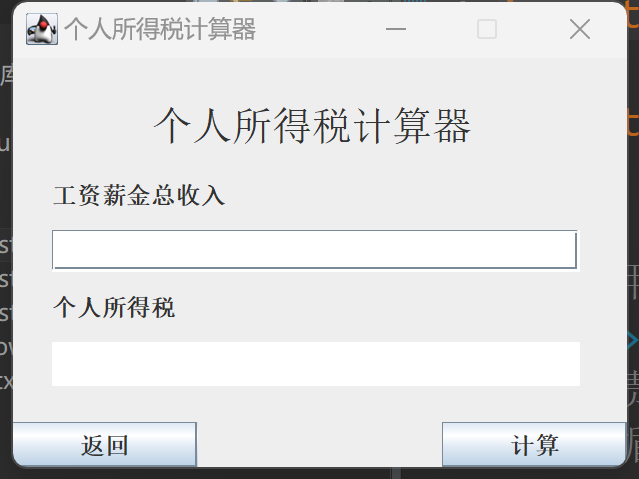
\includegraphics[height=0.15\textheight]{figure/GUITest.jpg}
            \vspace{.03\textheight}
            \caption{界面测试结果}
        \end{minipage}
        \begin{minipage}{.5\linewidth}
            \centering
            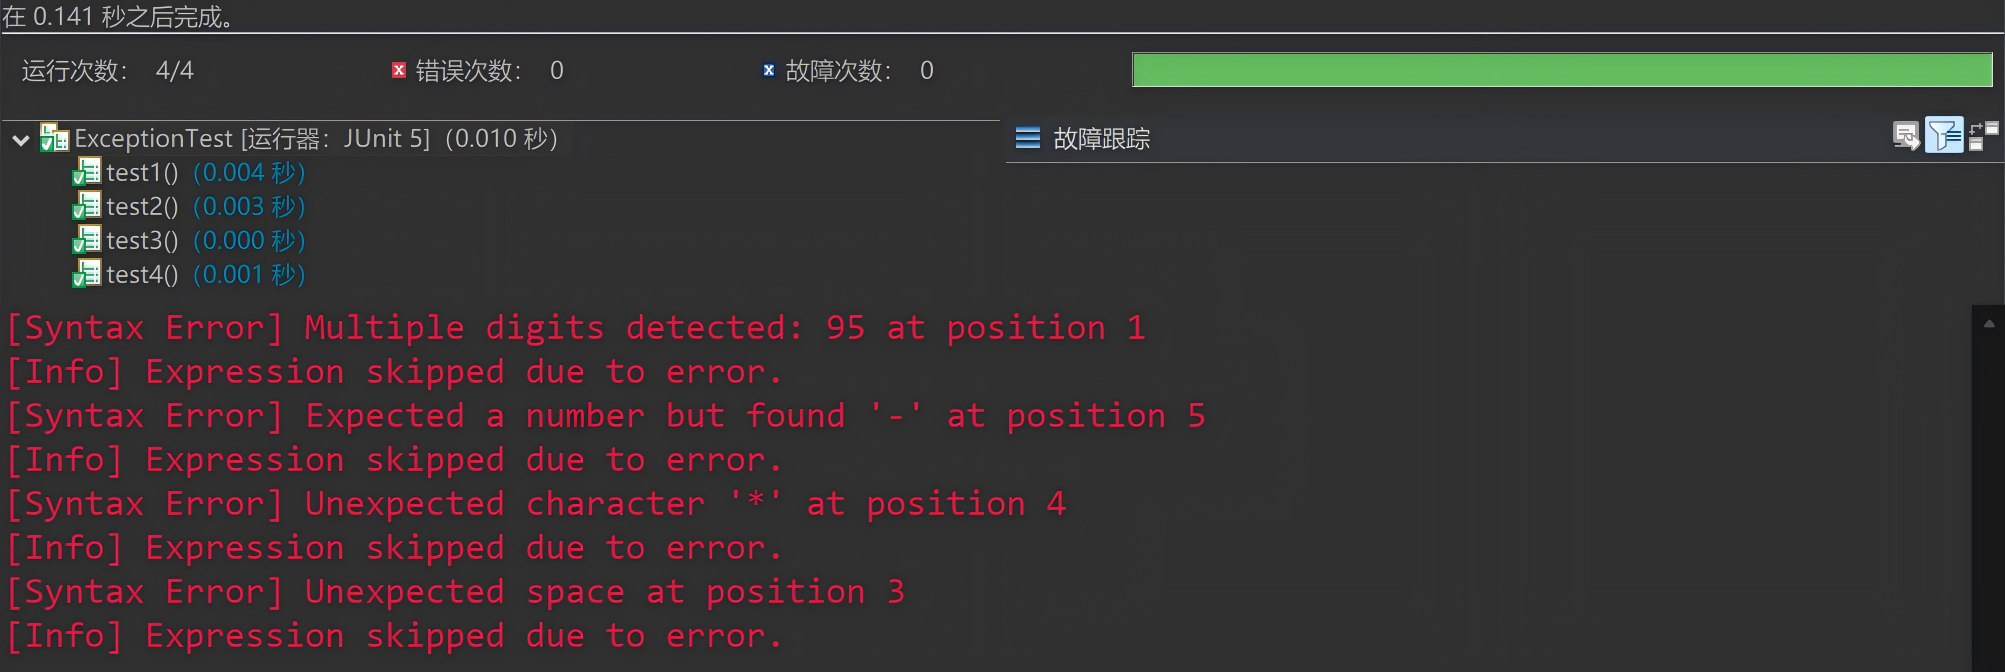
\includegraphics[height=0.21\textheight]{figure/ExceptionTest.png}
            \caption{异常处理测试结果}
        \end{minipage}
    \end{figure}

    \section{总结与思考}

    本项目成功设计并实现了一款可调整个人所得税起征点及税率表的计算器,具备完整的功能模块,包括数据存储、业务逻辑计算、用户界面交互及异常处理等。测试结果表明,该系统能够准确计算税额,并在各种输入条件下保持稳定性。

    然而,由于数据库当前仅能安装在本机内,数据存储仍依赖于本地文件,这在一定程度上限制了数据管理的灵活性和可扩展性。因此,未来可以进一步优化数据库的输入输出机制,以提升数据的存取效率和管理能力。

    尽管本项目的实现过程较为简单,但它作为工程化开发的入门项目,涵盖了从需求分析、系统架构设计到异常处理与测试验证的完整流程,为后续更复杂的工程实践提供了宝贵的经验。未来,项目可以考虑引入云端存储、自动更新税率等功能,以增强其实用性与可维护性。
    
    \let\cleardoublepage\clearpage
    
    \begin{thebibliography}{99}
        \bibitem{ref1} 沐言科技\ 李兴华.\ Java编程\ 从入门到实践[M].\ 第1版.\ 安徽:中国水利水电出版社,\ 2021.
        \bibitem{ref2} 中华人民共和国中央人民政府.\ 中国政府网站内搜索:个人所得税[EB/OL].\ [2025-03-01].\ https://sousuo.www.gov.cn/sousuo/search.shtml?code=17da70961a7\&dataTypeId=\ 107\&searchWord=\%E4\%B8\%AA\%E4\%BA\%BA\%E6\%89\%80\%E5\%BE\%97\%E7\%A8\%8E.
    \end{thebibliography}

\end{document}
